\documentclass{standalone}
\usepackage{pgfplots}
\pgfplotsset{compat=1.18}

\begin{document}
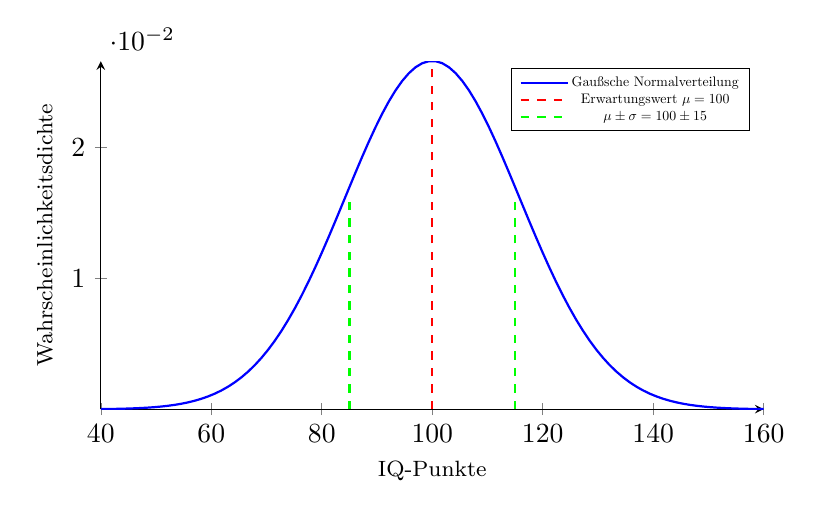
\begin{tikzpicture}
\begin{axis}[
    axis lines = left,
    xlabel = {\footnotesize IQ-Punkte},
    ylabel = {\footnotesize Wahrscheinlichkeitsdichte},
    samples=100,
    domain=40:160,
    height=6cm,
    width=10cm,
    no markers,
    every axis plot/.append style={thick},
    legend style = {
        nodes={scale=0.5}
    }
]

    \addplot [blue] {1/(15*sqrt(2*pi)) * exp(-((x-100)^2)/(500))};
    \addlegendentry{Gaußsche Normalverteilung}

    \draw [red, thick, dashed] (axis cs:100, 0) -- (axis cs:100, 0.0266);
    \addlegendimage{red, thick, dashed}
    \addlegendentry{Erwartungswert $\mu=100$}

    \pgfplotsinvokeforeach{85, 115} {
         \draw [green, thick, dashed] (axis cs:#1, 0) -- (axis cs:#1, 0.016);
    }

    \addlegendimage{green, thick, dashed}
    \addlegendentry{$\mu \pm \sigma = 100 \pm 15$}


\end{axis}
\end{tikzpicture}
\end{document}